\documentclass[acmsmall,nonacm,screen]{acmart}

% acmart provides graphicx, booktabs, hyperref, xcolor, url, amsmath.
\usepackage{amssymb}
\usepackage{multirow}

\graphicspath{{figures/}}

% "nonacm" strips the ACM publication apparatus (copyright/address footnotes,
% reference format, journal volume/issue/DOI strip) for a clean draft.
\settopmatter{printacmref=false}
\acmJournal{TRETS}

% Number supplementary floats S1, S2, ... so they are unambiguous from the
% main paper, which refers to them by these labels.
\renewcommand{\thefigure}{S\arabic{figure}}
\renewcommand{\thetable}{S\arabic{table}}

\begin{document}

\title{Supplementary Material for \\ ``Speculative GHR Forwarding: Eliminating Stale Branch-Predictor State in Deep FPGA Pipelines''}

\author{Devansh Joshi}
\affiliation{%
  \institution{The University of Texas at Austin}
  \department{Department of Electrical and Computer Engineering}
  \city{Austin}
  \state{Texas}
  \country{USA}}
\email{devansh.jos@utexas.edu}

\author{Shafin Ula}
\affiliation{%
  \institution{The University of Texas at Austin}
  \department{Department of Electrical and Computer Engineering}
  \city{Austin}
  \state{Texas}
  \country{USA}}
\email{shafin.ula@utexas.edu}

\maketitle

\noindent
This supplement collects corroborating figures and one modeled table referenced
from the main paper. All data are reproduced from the same measured runs; nothing
here is required to follow the main argument, which is why these floats are placed
out of line. Section numbers (S\ldots) and float labels (Fig.~S\ldots, Table~S\ldots)
match the citations in the main text.

\section{Area Scaling with Depth}
\label{sup:area}
Figure~\ref{fig:area} shows the slice LUT and flip-flop growth across the five
pipeline depths. The 4-to-8-stage increase is 622 LUTs (8.6\%) and 638 FFs (7.9\%);
DSP usage is constant at 12 blocks. The growth is gradual and sub-linear in the
added pipeline registers, because the dominant cost is the shared functional-unit
logic (ALU, MDU, register file), identical across depths; only the inter-stage
registers and the slightly larger forwarding/hazard logic grow.

\begin{figure}[h]
\centering
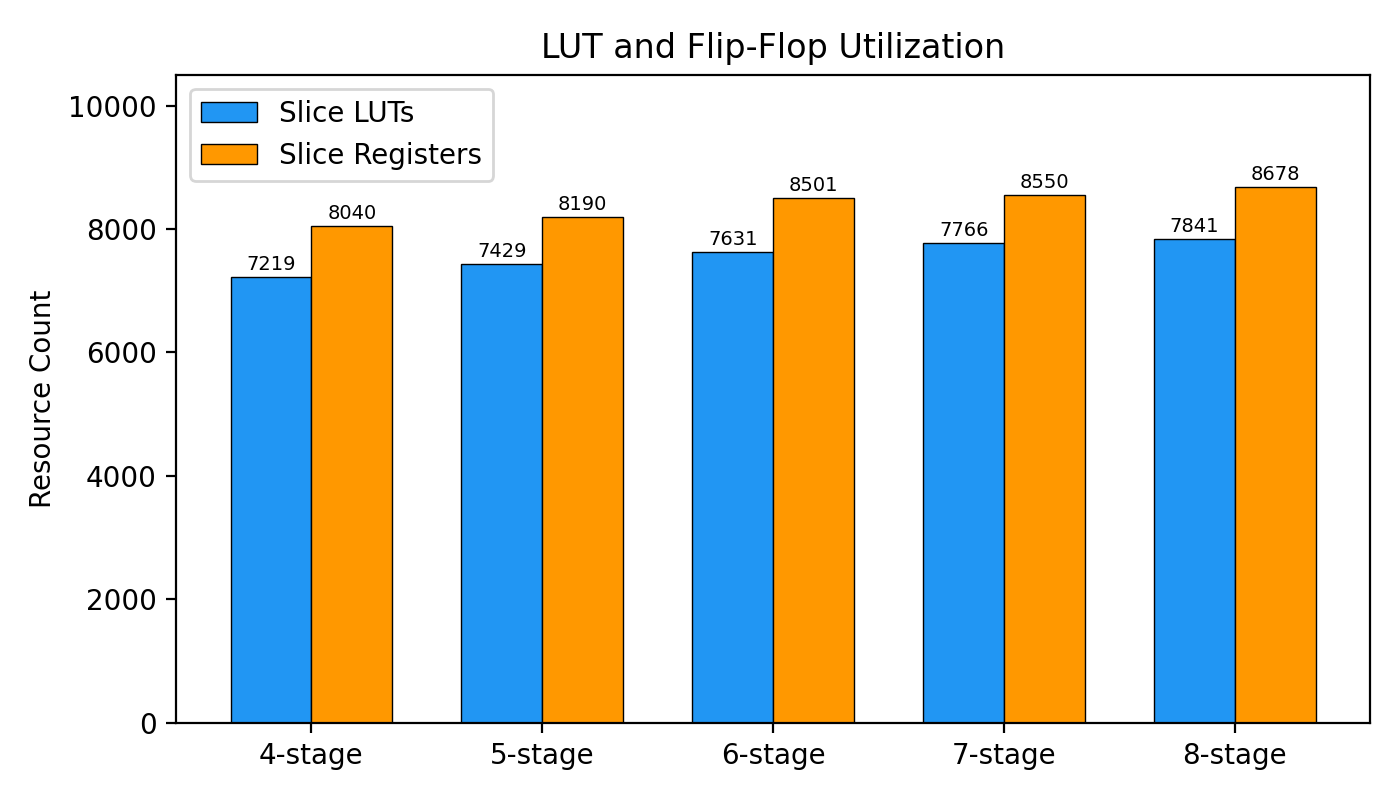
\includegraphics[width=0.7\columnwidth]{area_comparison.png}
\caption{Slice LUT and flip-flop utilization across pipeline depths on Artix-7 XC7A35T. The 4-to-8-stage increase is 622 LUTs (8.6\%) and 638 FFs (7.9\%); DSP usage is constant at 12 blocks.}
\label{fig:area}
\end{figure}

\section{CPI Model Residuals}
\label{sup:cpiresid}
Figure~\ref{fig:cpiresid} plots the CPI model residuals (measured minus predicted)
across depths. They have mean 0 and standard deviation 0.038\,CPI with no
depth-dependent pattern; the largest residual ($+$0.086) is on 6-stage CoreMark,
reflecting the smooth $M_w(D)$ slightly under-capturing the depth-6 misprediction jump.

\begin{figure}[h]
\centering
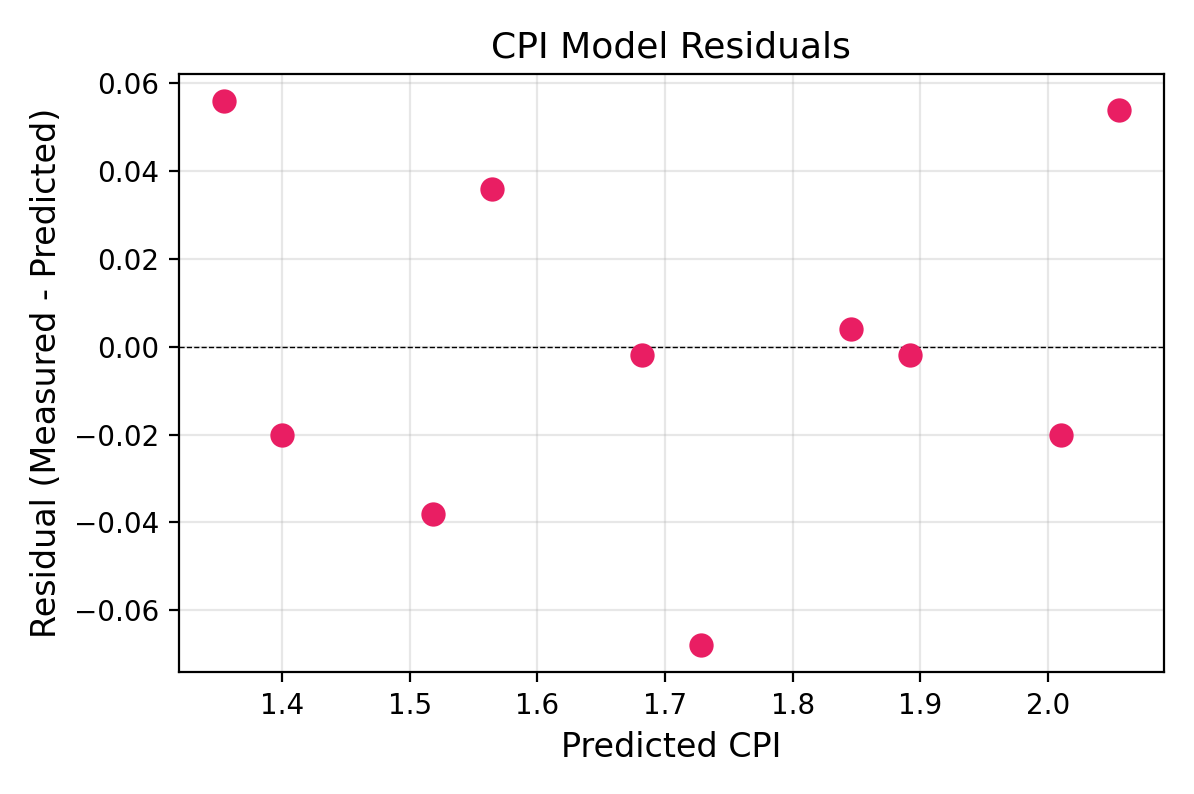
\includegraphics[width=0.7\columnwidth]{cpi_residuals.png}
\caption{CPI model residuals (measured minus predicted) across depths. Mean 0, standard deviation 0.038\,CPI, with no depth-dependent pattern; the largest residual ($+$0.086) is on 6-stage CoreMark.}
\label{fig:cpiresid}
\end{figure}

\section{BRAM Instruction Memory Effect}
\label{sup:bram}
Figure~\ref{fig:bram} compares $F_{\max}$ with LUT-RAM versus BRAM instruction memory
across the five depths. With BRAM the deep tier rises to 121.5\,MHz (6-stage),
120.9\,MHz (7-stage), and 121.2\,MHz (8-stage); the IF1/IF2 split absorbs the BRAM's
1-cycle read latency, so the 7/8-stage rise to near the 6-stage, while the shallow
tier holds (4-stage 69.3, 5-stage 73.7\,MHz). Mapping to BRAM shifts frequency but
not the CPI ordering, so the 6-stage stays the throughput optimum.

\begin{figure}[h]
\centering
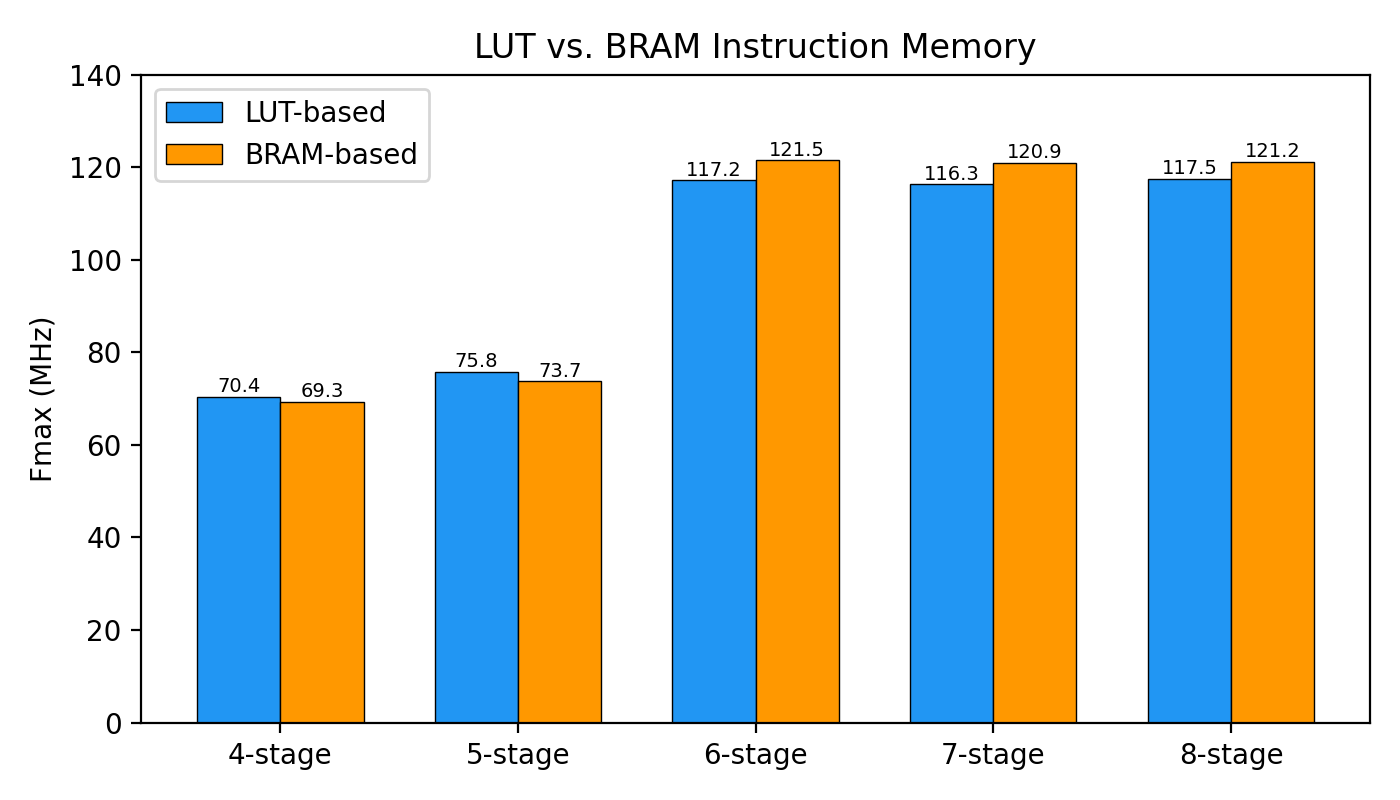
\includegraphics[width=0.7\columnwidth]{bram_comparison.png}
\caption{$F_{\max}$ with LUT-RAM versus BRAM instruction memory across the five depths. The IF1/IF2 split absorbs the BRAM read latency, so the 7/8-stage rise to near the 6-stage; the 4/5-stage tier is unchanged.}
\label{fig:bram}
\end{figure}

\section{Power and Efficiency}
\label{sup:power}
Figure~\ref{fig:power} shows the on-chip power breakdown across depths under
workload-specific (CoreMark SAIF) switching activity, and Figure~\ref{fig:efficiency}
the resulting efficiency. Total power falls with depth from 0.235\,W (4-stage) to
0.217\,W (8-stage) because lower IPC reduces average toggling. The 6-stage is the
most energy-efficient depth at 286\,MIPS/W, as well as the highest-throughput. These
are Vivado vector-based estimates at ``Medium'' confidence, not physical measurements;
we rely on the relative ordering across depths, not the absolute watts.

\begin{figure}[h]
\centering
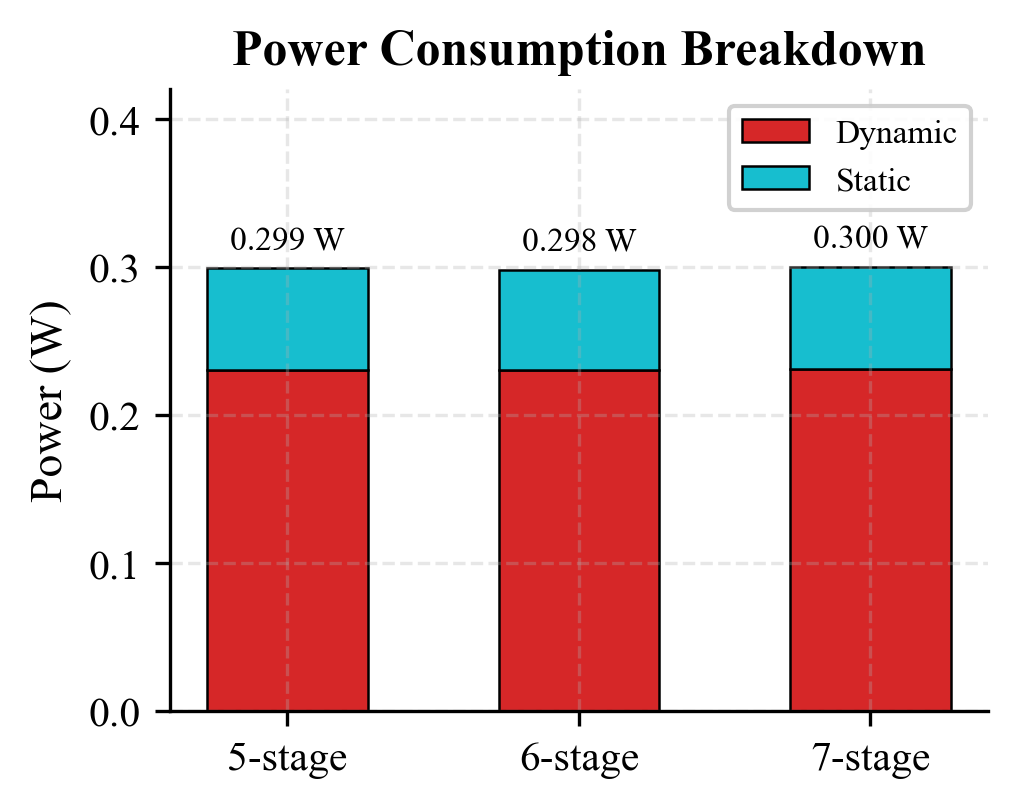
\includegraphics[width=0.7\columnwidth]{power_comparison.png}
\caption{On-chip power (dynamic and static) across the five depths under workload-specific (CoreMark SAIF) switching activity. Total power falls with depth as lower IPC reduces average toggling.}
\label{fig:power}
\end{figure}

\begin{figure}[h]
\centering
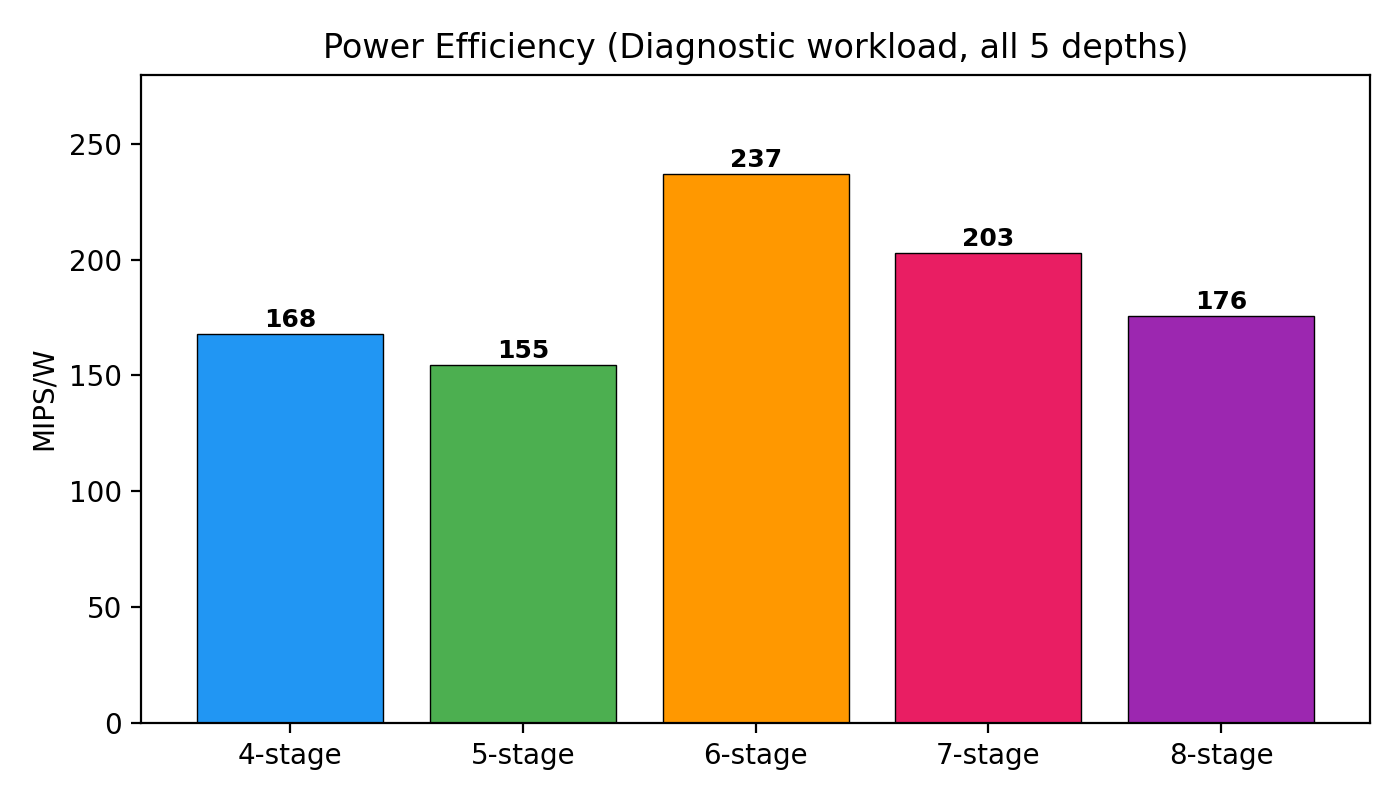
\includegraphics[width=0.7\columnwidth]{efficiency_comparison.png}
\caption{Power efficiency (MIPS/W) across the five depths, from SAIF-based power and CoreMark throughput. The 6-stage is the most efficient at 286\,MIPS/W.}
\label{fig:efficiency}
\end{figure}

\section{Cache-Miss Sensitivity (Modeled)}
\label{sup:cache}
Table~\ref{tab:cache_sensitivity} works the 7-stage CoreMark case through four
modeled cache-miss scenarios. SGF's absolute cycle saving (159{,}932 cycles) is
miss-rate-independent, so its relative benefit shrinks as memory stalls grow to
dominate CPI. These are analytical projections, not measured against a real hierarchy.

\begin{table}[h]
\centering
\caption{SGF throughput improvement under modeled cache-miss rates (7-stage CoreMark). The absolute cycle saving from SGF (159{,}932 cycles) is constant, so the relative improvement decreases as memory stalls grow to dominate CPI.}
\label{tab:cache_sensitivity}
\small
\begin{tabular}{@{}lccccc@{}}
\toprule
\textbf{Miss scenario} & \textbf{Miss CPI} & \textbf{Total CPI (base)} & \textbf{Total CPI (SGF)} & \textbf{$\Delta$CPI} & \textbf{Rel.\ improvement} \\
\midrule
No misses (this study)      & 0    & 2.02 & 1.96 & $-$0.06 & 3.0\% \\
1\% miss, 20-cycle penalty  & 0.20 & 2.22 & 2.16 & $-$0.06 & 2.7\% \\
2\% miss, 50-cycle penalty  & 1.00 & 3.02 & 2.96 & $-$0.06 & 2.0\% \\
5\% miss, 100-cycle penalty & 5.00 & 7.02 & 6.96 & $-$0.06 & 0.9\% \\
\bottomrule
\end{tabular}
\end{table}

\section{Published-Cores Context}
\label{sup:published}
Figure~\ref{fig:published} places our five variants against published Artix-7 RISC-V
soft cores. It is included only to confirm our research vehicle sits in a realistic
design-space region (70--118\,MHz); the cores differ in ISA subset, execution model,
predictor, and memory, so their frequency gaps reflect those confounders, not pipeline
depth. We make no cross-project performance claim.

\begin{figure}[h]
\centering
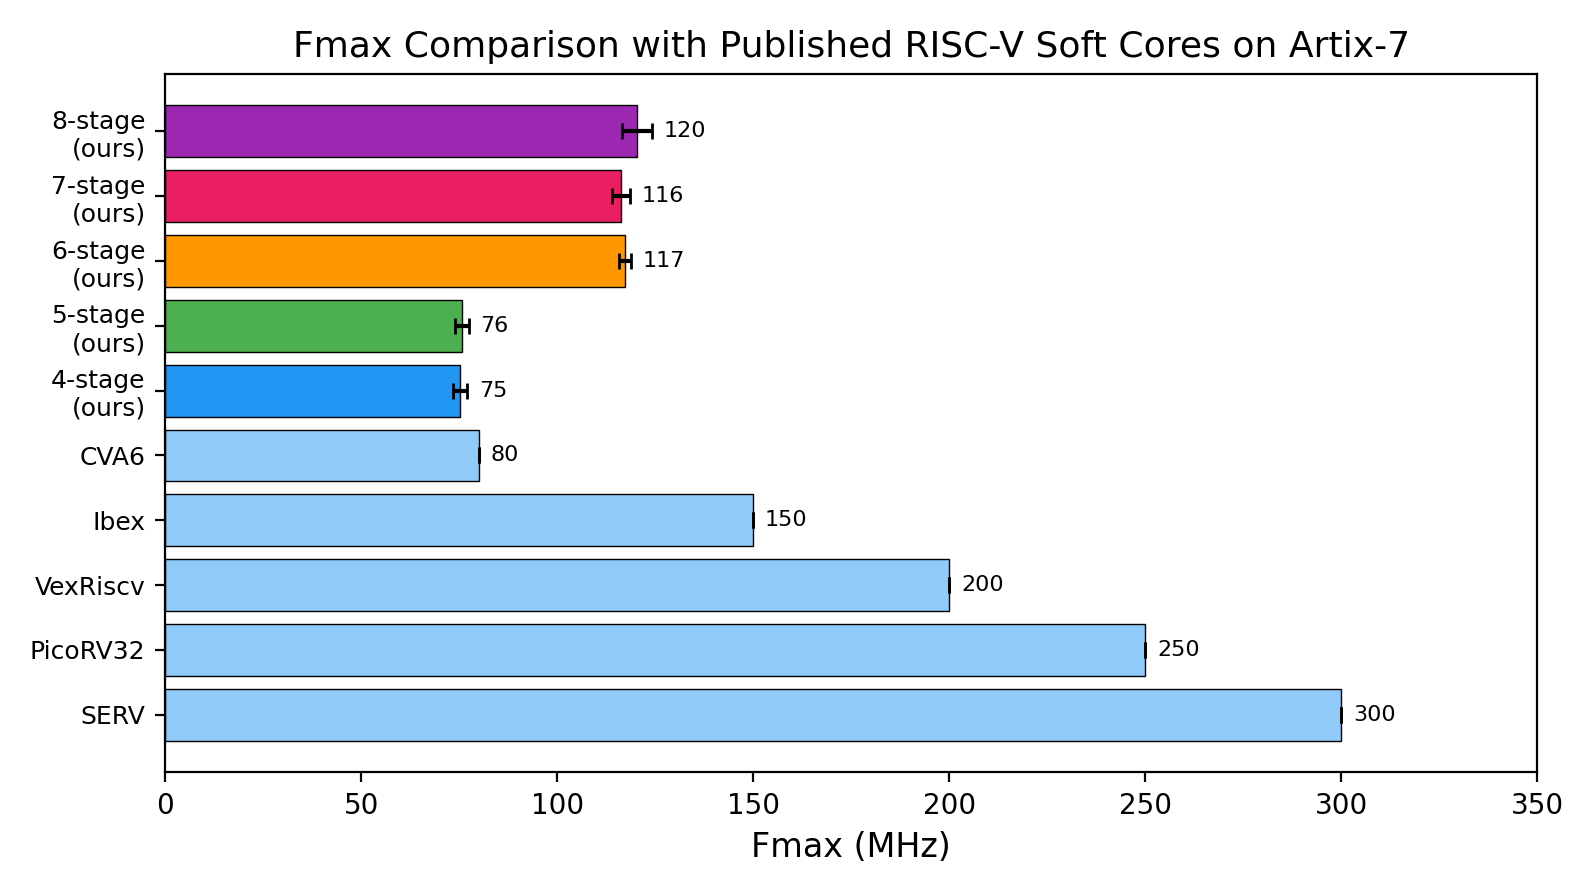
\includegraphics[width=0.7\columnwidth]{published_cores_comparison.png}
\caption{$F_{\max}$ of our five variants against published Artix-7 RISC-V soft cores. Included only to confirm our research vehicle sits in a realistic design-space region; the cores differ in too many variables to support a cross-project performance comparison.}
\label{fig:published}
\end{figure}

\section{CoreMark Detail Across Depths}
\label{sup:coremark}
Table~\ref{tab:coremark} gives the full official CoreMark figures across the five
depths. The CPI and misprediction columns also appear in the main paper; the cycle
and CoreMark/MHz rows are reported here in full.

\begin{table}[h]
\centering
\caption{Official EEMBC CoreMark results across the five pipeline depths (10 iterations, PERFORMANCE\_RUN). All variants execute identical instruction counts (2{,}893{,}145) and branch counts (719{,}810). Cycles and mispredictions are from RTL simulation; CoreMark/MHz uses the post-place-and-route $F_{\max}$.}
\label{tab:coremark}
\small
\begin{tabular}{@{}lccccc@{}}
\toprule
\textbf{Metric} & \textbf{4-stg} & \textbf{5-stg} & \textbf{6-stg} & \textbf{7-stg} & \textbf{8-stg} \\
\midrule
Cycles          & 4{,}481{,}534 & 4{,}724{,}937 & 5{,}310{,}372 & 5{,}856{,}929 & 6{,}323{,}069 \\
Mispredictions  & 145{,}735 & 145{,}735 & 154{,}077 & 147{,}760 & 147{,}760 \\
Mispredict rate & 20.2\%    & 20.2\%    & 21.4\%    & 20.5\%    & 20.5\% \\
CPI             & 1.54      & 1.63      & 1.83      & 2.02      & 2.18 \\
CoreMark/MHz    & 2.23      & 2.12      & 1.88      & 1.71      & 1.58 \\
\bottomrule
\end{tabular}
\end{table}

\section{CoreMark CPI Ablation}
\label{sup:ablation}
Table~\ref{tab:ablation} decomposes CoreMark CPI into the four additive terms of the
main paper's CPI model equation at each depth. The summed prediction matches measured
CPI within the model residual ($\leq$0.09).

\begin{table}[h]
\centering
\caption{CPI ablation for CoreMark: decomposition into the architectural cost components of the CPI model equation (main paper) at each pipeline depth. Each row is one term. The sum matches measured CPI within the model residual ($\leq$0.09).}
\label{tab:ablation}
\small
\begin{tabular}{@{}lccccc@{}}
\toprule
\textbf{CPI component} & \textbf{4-stg} & \textbf{5-stg} & \textbf{6-stg} & \textbf{7-stg} & \textbf{8-stg} \\
\midrule
Ideal throughput                       & 1.00 & 1.00 & 1.00 & 1.00 & 1.00 \\
Branch flush ($M \cdot P / N$)         & 0.10 & 0.10 & 0.16 & 0.20 & 0.20 \\
Load-use stall ($\alpha \cdot L$)      & 0.00 & 0.15 & 0.15 & 0.15 & 0.22 \\
IF2 bubble ($\beta \cdot B \cdot f_b$) & 0.00 & 0.00 & 0.00 & 0.28 & 0.28 \\
Workload base ($\gamma_w$)             & \multicolumn{5}{c}{0.45 (depth-invariant)} \\
\midrule
\textbf{Model prediction}              & \textbf{1.55} & \textbf{1.70} & \textbf{1.76} & \textbf{2.08} & \textbf{2.15} \\
\textbf{Measured CPI}                  & \textbf{1.54} & \textbf{1.63} & \textbf{1.83} & \textbf{2.02} & \textbf{2.18} \\
\bottomrule
\end{tabular}
\end{table}

\section{Mechanism-B Susceptibility by Inter-Branch Distance}
\label{sup:ibd}
Table~\ref{tab:ibd} classifies the seven workloads by inter-branch distance (IBD) and
observed Mechanism~B behavior. The two workloads that exhibit Mechanism~B (CoreMark,
statemate) have IBD~$\leq$~8.4 and data-dependent outcomes; workloads with larger IBD
or highly biased outcomes show no depth-dependent variation.

\begin{table}[h]
\centering
\caption{Mechanism~B susceptibility classified by inter-branch distance (IBD) and branch outcome predictability.}
\label{tab:ibd}
\small
\begin{tabular}{@{}lccc@{}}
\toprule
\textbf{Workload} & \textbf{IBD} & \textbf{Outcome type} & \textbf{Mech.~B?} \\
\midrule
CoreMark   & 4.0  & Data-dependent  & Yes (+5.7\%) \\
statemate  & 8.4  & Data-dependent  & Yes (+10\%) \\
edn        & 8.8  & Mixed           & No \\
aha-mont64 & 8.7  & Biased loops    & No \\
Diagnostic & 3.8  & Structured      & No \\
Dhrystone  & 7.3  & Structured      & No \\
crc32      & 23.0 & Highly biased   & No \\
\bottomrule
\end{tabular}
\end{table}

\section{Pipeline Structure and Hazard Costs}
\label{sup:hazard}
Table~\ref{tab:hazard} lists the per-event hazard costs across the five depths
(architectural parameters, not measured data). The bottom row, predictor update
latency, is the central variable for Mechanism~B.

\begin{table}[h]
\centering
\caption{Pipeline structure and per-event hazard costs across depths (architectural parameters, not measured data). Predictor update latency (bottom row) is the central variable for Mechanism~B.}
\label{tab:hazard}
\small
\begin{tabular}{@{}lccccc@{}}
\toprule
\textbf{Property} & \textbf{4-stg} & \textbf{5-stg} & \textbf{6-stg} & \textbf{7-stg} & \textbf{8-stg} \\
\midrule
Pipeline registers        & 3 & 4 & 5 & 6 & 7 \\
Forwarding sources        & 1 & 2 & 3 & 3 & 3 \\
Load-use stall            & 0 & 1\,cy & 1\,cy & 1\,cy & 1--2\,cy \\
Branch penalty            & 2\,cy & 2\,cy & 3\,cy & 4\,cy & 4\,cy \\
IF2 prediction bubble     & 0 & 0 & 0 & 1\,cy & 1\,cy \\
Predictor update latency  & 2 & 2 & 3 & 4 & 4 \\
\bottomrule
\end{tabular}
\end{table}

\end{document}
